\documentclass[a4paper,10pt]{report}

\usepackage[latin1]{inputenc}
\usepackage[T1]{fontenc}
\usepackage[francais]{babel}
\usepackage{greekctr}
\usepackage{graphicx}
\usepackage{url}
\usepackage{amssymb}
\usepackage{graphicx}
\usepackage[usenames]{color}
\usepackage[left=1.0cm,top=1.5cm,right=0.5cm,nohead,nofoot]{geometry}
\usepackage{array}
\usepackage{longtable}


\newcommand{\SP}{\tiny~\\}
\newcommand{\SPb}{\footnotesize\hspace{0.5cm}~&\footnotesize\hspace{2.5cm}~&\\}
\newcommand{\comment}[1]{} 


%
% Commands for Experience Table
%
\newcommand\XpLine[2]{
\SP
&
	\begin{tabular}{p{3cm}}
		#1
	\end{tabular}
	&
	\begin{tabular}{p{12.5cm}}
		#2
	\end{tabular} \\
}

\newcommand\XpTitle[3]{
\XpLine
	{	\textbf{#1}}
	{	\textbf{#2} \\
		\textit{#3}
	}
}		

\newcommand\XpItem[6]{
\XpLine
	{
		\textbf{#1}\\
		�\\
		\textbf{#2}
	}
	{
		\textbf{#3} (#4)\\
		\textbf{Projet} : #5\\
		\textbf{Mission} : #6
	}
}

\newcommand\XpItemEn[6]{
\XpLine
	{
		\textbf{#1}\\
		to\\
		\textbf{#2}
	}
	{
		\textbf{#3} (#4)\\
		\textbf{Project} : #5\\
		\textbf{Mission} : #6
	}
}


%
% Commands for Formation
%


\newcommand\FormationLine[2]{

\SP
&
	\begin{tabular}{p{3cm}}
		#1
	\end{tabular}
	&
	\begin{tabular}{p{12.5cm}}
		#2
	\end{tabular} \\
}


\newcommand\FormationItem[3]
{

\FormationLine
	{\textbf{#1}}
	{\textbf{#2} \\
	 #3} \\	 
}

%
% Commands for Comp
%

\newcommand\SkillLine[2]{

\SP
&
	\begin{tabular}{p{3cm}}
		#1
	\end{tabular}
	&
	\begin{tabular}{p{12.5cm}}
		#2
	\end{tabular} \\
}


\newcommand\SkillItem[2]
{

\SkillLine
	{\textbf{#1}}
	{#2}
}

\newcommand\Adress[0]{
	\begin{tabular}{ll}
		\multicolumn{2}{l}{\textbf{Arnaud DEMARCQ}}				\\
		\multicolumn{2}{l}{Immeuble \textit{Le Saint Romain}}	\\
		\multicolumn{2}{l}{Entr�e D-E}						\\
		\multicolumn{2}{l}{63 boulevard de la madeleine}	\\
		\multicolumn{2}{l}{06000 Nice (FRANCE) }			\\
		\textbf{Tel} :	&	+33 682 618 213				\\
		\textbf{Mail} :	&	demarcq@iie.cnam.fr			\\
						&	arnaud.demarcq@gmail.com 	\\
	\end{tabular}
}


%
% Document
% 




\begin{document}

\begin{titlepage}

\begin{center}
\begin{tabular}{lcr}
		\Adress
	\begin{tabular}{ll}
			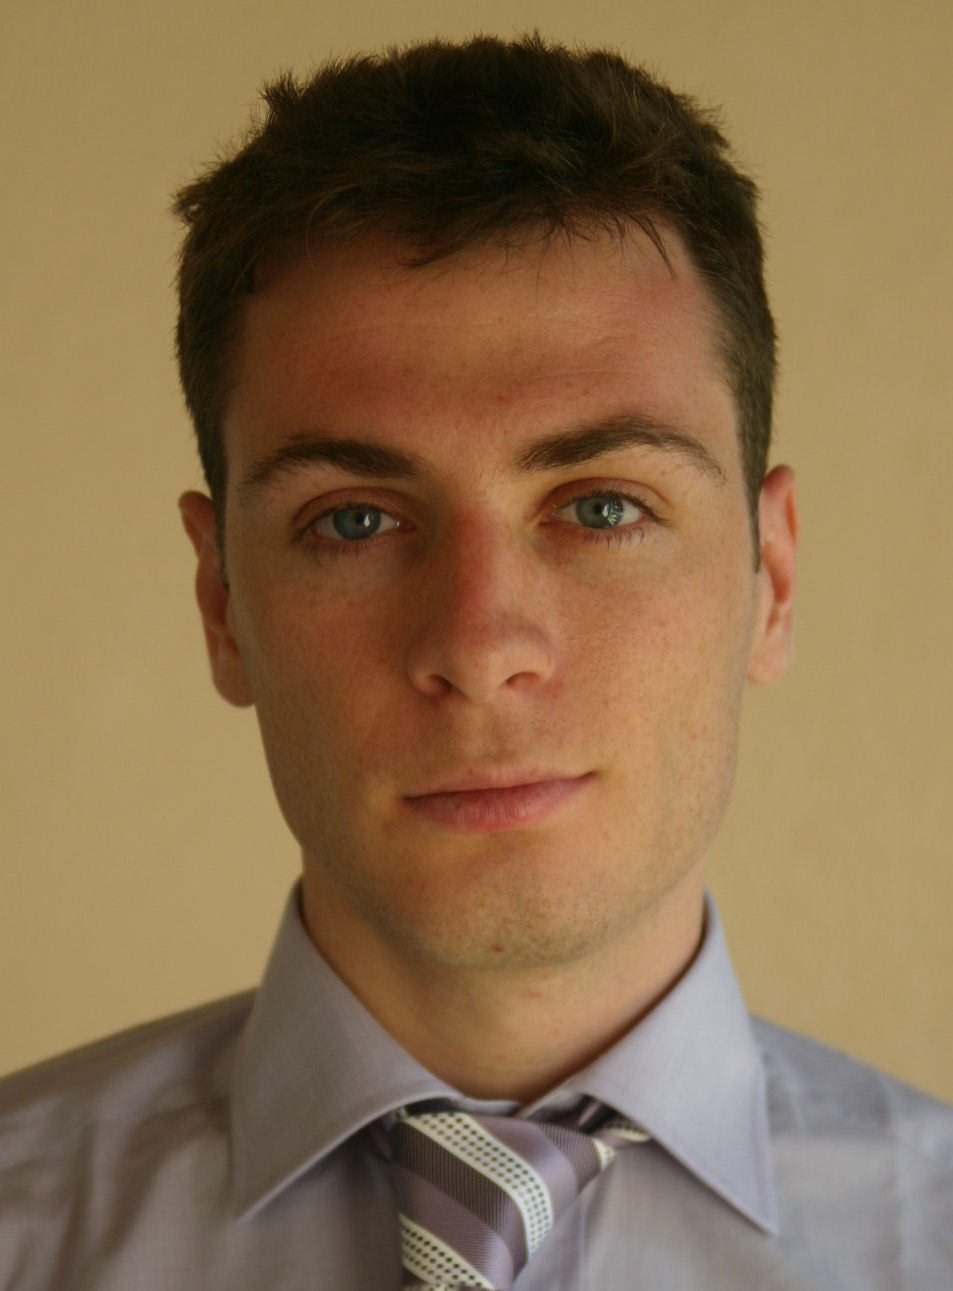
\includegraphics[width=75pt]{demarcq.jpg}
	\end{tabular}
	\begin{tabular}{l}
		Born the 27\up{th} April 1982 in Aix en Provence		\\
		French 		\\
		Bachelor					\\
		Driving Licence					\\
	\end{tabular}				
\end{tabular}


\end{center}

\textcolor{blue}{\uppercase{\textbf{Educational background  :}}}

\begin{tabular}{p{0.1cm} p{2cm} p{13.5cm}}
\FormationItem
	{2005}
	{Ing�nieur IIE (French Grande �cole of Computer Science) }
	{}
		
\FormationItem
	{2004}
	{Master d'Informatique Fondamentale in Marseille (Fundamental Computer Science)}
	{Options : \textit{Cryptography}, 
		\textit{Logic and Proof Fundamentals} and
		\textit{Large Database Environments}.}
		
\FormationItem
	{2004}
	{Master AMIB (Maths and Informatics for Biology)}
	{Done in parallel with the IIE}

	
\FormationItem
	{1999}
	{Baccalaur�at}
	{}

\end{tabular}		



\textcolor{blue}{\uppercase{\textbf{Professional experience :}}}

\begin{longtable}{p{0.1cm} p{3cm} p{12.5cm}}


\XpItemEn
	{February 2009}{Now}
	{Creation of the start up Business Inovative Solutions}{B.I.S}
	{Among with other former Experian Scorex employees, creation of this company for 
	creating, developing and selling Integration and BPM (Business  Process Management) software.}
	{Architecture, Pre Sales, Development}
	
\XpItemEn
	{November 2007}{February 2009}
	{Other Important Projects}
	{Experian Scorex}
	{Bank of America Europe , CUP (China), Alliance and Leicester  (UK), Swiss Card}
	{Technical Architecture, Customer training, project management,
		On site integration and performance testing, support.
		On site missions in China, Switzerland, UK.}
	
\XpItemEn
	{November 2007}{February 2009}
	{Universal Gateway}
	{Experian Scorex}
	{Internal Product}
	{Internal Promotion of the product, Training, Development of modules}

\XpTitle
	{July 2008}
	{Appointed Software Development Lead}
	{Technical Leader in a team of 5 persons, (Responsibility  of assignation, priorities, reporting),
		Responsibility  of technical and architectural choices for internally developed  solutions.
		Internal Promotion of GTC team architectural choices.
		Architectural and Technical Leadership.}

\XpItemEn
	{November 2007}{July 2008}
	{Barclays Bank}
	{Experian Scorex}
	{Implementation of the core banking solution for Barclays Bank, for all African countries, India and Pakistan}
	{Technical Architecture, Development  of the Credit Bureaus interfaces, On site Training, Support and Performance
	Testing}

\XpItemEn
	{November 2007}{July 2008}
	{SBSA}
	{Experian Scorex}
	{Implementation of the core banking solution for SBSA (Standard Bank South Africa), first South African Bank}
	{Technical Architecture, Development of the Credit Bureaus interfaces, On site Training, Support and Performance
	Testing}

\XpTitle
	{November 2007}
	{Joined Experian Scorex as Technical Consultant}
	{In the Global Technical  Consultency Team (GTC), a Technical Consultant works on projects delivered by Experian from the presales
	to the delivery, act as a third line of support for the Company Software, and takes care of punctual Training missions}
	
\XpItemEn
	{March 2007}{November 2007}
	{Experian Scorex}
	{Capgemini}
	{Support, Consultancy  and Development  around the core banking software \textit{Transact SM} }
	{Within the GTC Team(Global Technical  Consultancy  ), Development of integration solutions for Transact }

\XpItemEn
	{February 2006}{March 2007}
	{Jax \textit{ACOSS}}
	{Capgemini}
	{Realization of a application for the replacement of Tuxedo in the ACOSS environment, in order to allow 
	the interfacing with other Java, C++ and Cobol software,.}
	{Within a team of 3 persons, Development , tests and maintenance of the application}
	

\XpItemEn
	{July}{December 2005}
	{ALMA \textit{Swisscom}}
	{Capgemini}
	{Realization  of a module allowing to manage SWISSCOM specific equipments through TEMIP.
	Data retrieved  by these equipments are centralized by a Gateway that analyses that broadcast them
	as ascii string to the developed  Access Module (AM) }
	{ Functional  and Integration Tests, realization of simulators allowing to tesst different modules independently	}
		
\XpTitle
	{Juillet 2005}
	{Join Capgemini Nice}
	{}		
\end{longtable}		






\textcolor{blue}{\textbf{\uppercase{Skills :}}}

\begin{tabular}{p{0.1cm} p{2cm} p{13.5cm}}

\SkillItem
	{Java/J2EE \newline Architect }
	{Solid Knowledge on various frameworks sur as Spring, Hibernate, OSGI ...}
	
\SkillItem
	{Develo-\newline  pement}
	{JAVA/J2EE, C, C++, Visual Basic, Perl
		CAML, FORTRAN, PHP, HTML, ASM}

\SkillItem
	{Project \newline Management}
	{Project Management in an International Environement.}
	
\SkillItem
	{English}
	{Fluent \\ \textit{875 points at the Toeic}}
	
\SkillItem
	{operating \newline Systems}
	{Linux/Unix/Aix, Windows, OSX ...}\\

\end{tabular}		


~\\

\textcolor{blue}{\uppercase{\textbf{Extra professional activities  :}}}

\begin{tabular}{llp{13.5cm}}
\SP
&	\begin{tabular}{l}
		\small \textbf{Litterature}
	\end{tabular}
&	\begin{tabular}{l}
		Science Fiction, fantasy ...
	\end{tabular}\\
~\\

&	\begin{tabular}{l}
		\small \textbf{Programming}
	\end{tabular}
&	\begin{tabular}{l}
		Small Programs (Games, small utilities) \\
		Pocs (proofs of concept) on recents java frameworks (wicket, OSGI, spring 3 ...) \\
		Contributes to Open Sources Initiatives \\
	\end{tabular}\\
~\\
&	\begin{tabular}{l}
		\small \textbf{Sports}
	\end{tabular}
&	\begin{tabular}{l}
		Swim, ski, snow board ...\\
	\end{tabular}\\
~\\
&	\begin{tabular}{l}
		\small \textbf{Other }
	\end{tabular}
&	\begin{tabular}{l}
		Role playing Games
	\end{tabular}\\

\end{tabular}

\comment{\center{\tiny{\textbf{CV mis a jour le 21 Juin 2005}}}}

\end{titlepage}

\end{document}


